\documentclass[aspectratio=169, 15pt,usenames,dvipsnames]{beamer}


\usepackage[utf8]{inputenc}
\usepackage{fontspec}
\usepackage{sansmathfonts}
\usepackage{xcolor}
\usepackage{fontenc}
\usepackage{unicode-math}
\usepackage{listings}
\usepackage{cprotect}

\usepackage[makeroom]{cancel}

\usefonttheme{serif}
\usefonttheme{professionalfonts}


\usepackage[sfdefault,scaled=1.1]{FiraSans}
\usepackage{sourcecodepro}
\usepackage{graphicx}

\graphicspath{
    {themes/gd/images/},
    {images/}
}
\usepackage{themes/gd/beamerthemegd}
\usepackage{themes/gd/beamerinnerthemegd}
\usepackage{themes/gd/beamerouterthemegd}
\usepackage{themes/gd/beamercolorthemegd}



\graphicspath{
    {themes/gd/images/},
    {images/}
}

\setlength{\parskip}{1em}
\setbeamertemplate{footline}{%
   \raisebox{5pt}{\makebox[\paperwidth]{\hfill\makebox[10pt]{\scriptsize\insertframenumber}}}}

\title{The Streaming Data Platform\\\small as a heavy duty\\enterprise data marketplace\\\tiny when to use it in your project\\the case of MMA}
% \date[ISPN ’80]{27th International Symposium of Prime Numbers}
\author[Euclid]{Euclid of Alexandria \texttt{euclid@alexandria.edu}}


\begin{document}  
\begin{titlePage} 
	\titlepage        
\end{titlePage}
	
\begin{gdsw}
	\frametitle{Hello}
	\centering
\includegraphics[scale=2.3]{denis}
	\\Denis Golovachev		
\end{gdsw} 
\begin{gdsw}
	\frametitle{Hello}
	\centering
\includegraphics[height=0.6\textheight]{pikachu}
	\\Roman Zakharov [I don't have his photo, but this is quite close]
\end{gdsw} 	
\begin{gdsw}
	\centering
\includegraphics[scale=0.3]{gdlogo}
\end{gdsw}
\begin{gdsw}
	\frametitle{SPB}
	\centering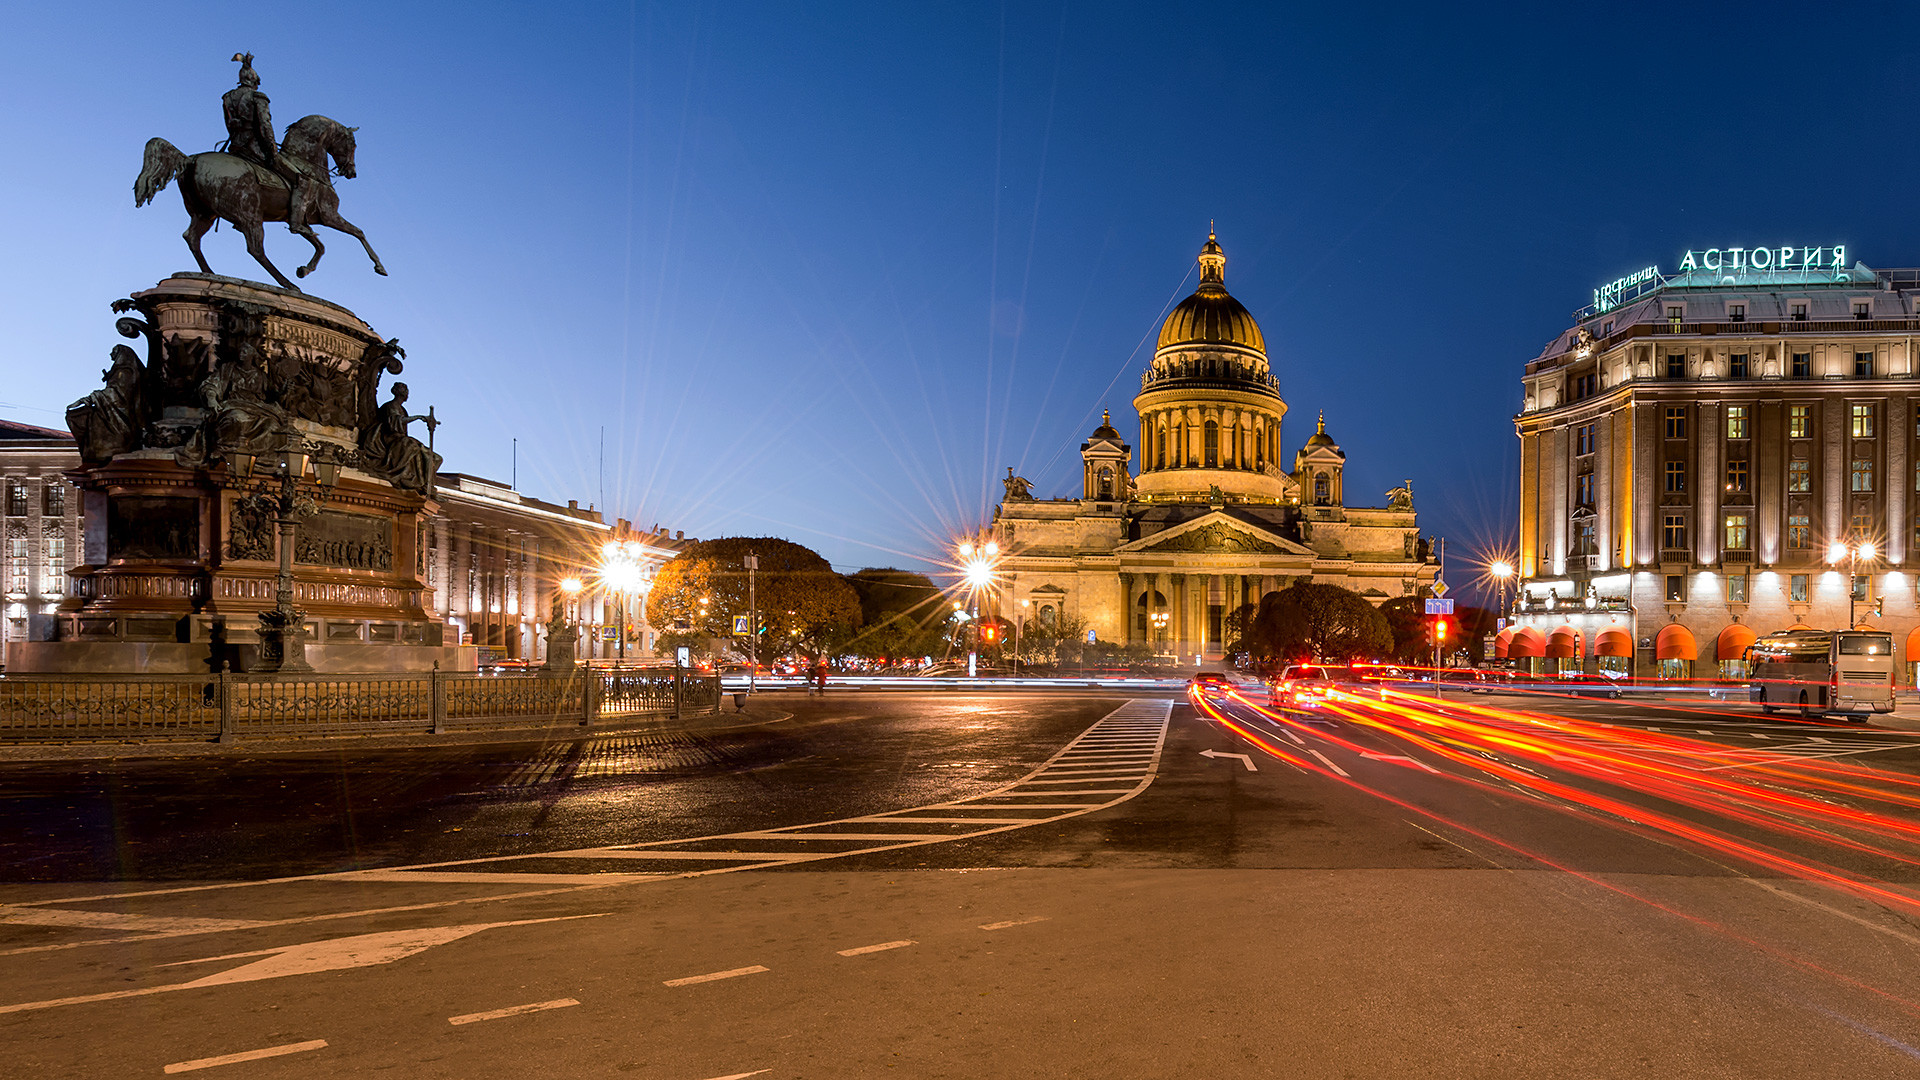
\includegraphics[height=0.7\textheight]{spb}
	\\Saint-Petersburg
\end{gdsw}
\begin{gdsw}
	\frametitle{KRK}
	\centering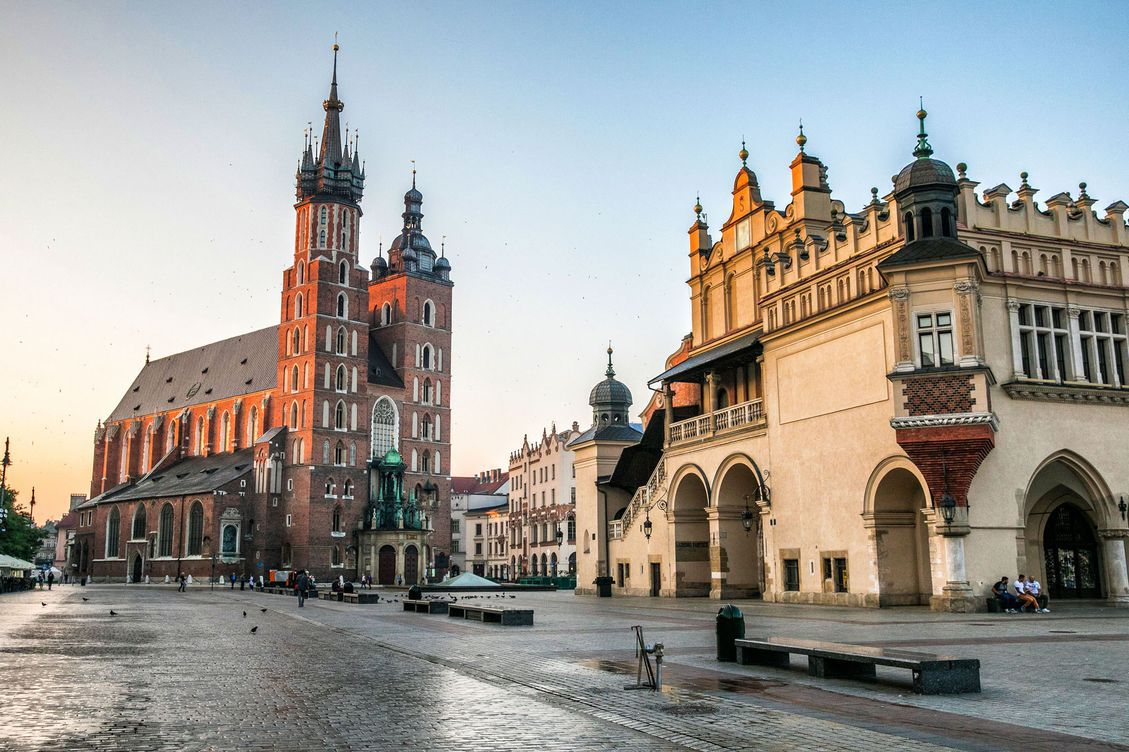
\includegraphics[height=0.7\textheight]{krakov}
	\\Krakov
\end{gdsw}
\begin{gdsw}
	\centering
\includegraphics[height=0.9\textheight]{bigdata} 
\end{gdsw}
\begin{gdsw}
	\centering
\includegraphics[height=0.7\textheight]{garchitect} 
	\par\LARGE
	Software Architect
\end{gdsw}
\begin{gdsw}
	\centering
\includegraphics[height=0.7\textheight]{analytics} 
	\par\LARGE
	Business Analytic
\end{gdsw}
\begin{gdsw}
	\frametitle{Data Streaming}
	\centering
\includegraphics[width=0.8\textwidth]{streaming} 
\end{gdsw}
\begin{gdsw}
	\centering\LARGE
	The Streaming Data Platform\\
	as a heavy duty enterprise data marketplace\\
	When to use it in your project.\\
	The case of MMA
\end{gdsw}
\begin{gdsw}
	\centering\LARGE
	{\bf The Streaming Data Platform}\\
	as a heavy duty enterprise data marketplace\\
	{\bf When to use it in your project.}\\
	The case of MMA
	\pause\\
	{\it\small MMA - Multichannel Marketing Automation}
\end{gdsw}
\begin{gdsw}
	\LARGE\centering Small Introduction to
	\centering
\includegraphics[width=0.8\textwidth]{bigdata}
	\par
	Streaming Platforms
\end{gdsw}
\begin{gdsw}
	\centering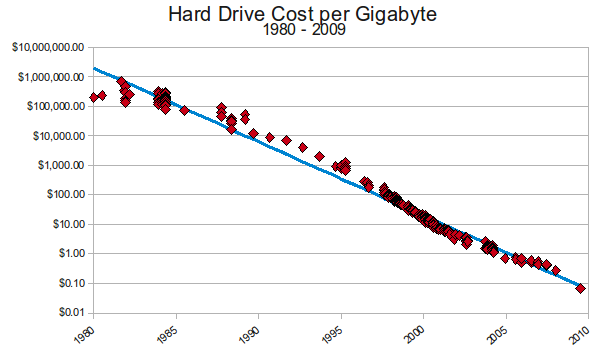
\includegraphics[height=0.6\textheight]{hdd-cost-2} 
	\par
	For the past 35+ years or so, hard drives prices have dropped, from around \$500,000 per gigabyte in 1981 to less than \$0.02 per gigabyte today
\end{gdsw}
\begin{gdsw}
	\centering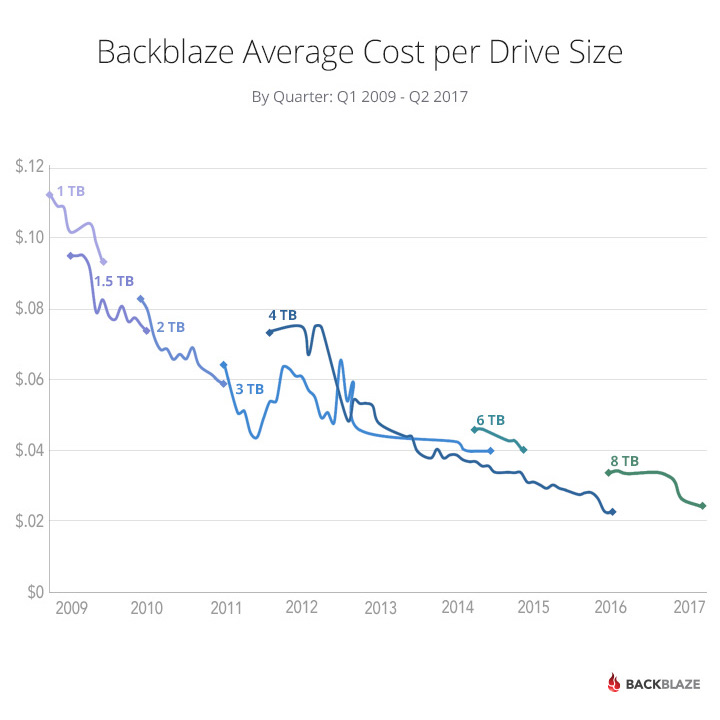
\includegraphics[height=0.6\textheight]{hdd-cost}\\
	\centering\tiny [https://www.backblaze.com/blog/hard-drive-cost-per-gigabyte/]
	\par\normalsize\centering\begin{itemize}
	\item 2010 year - countries could afford to store everything. i.e. USA PRIZM
	\item 2015 - big companies could afford to store everything. i.e. Google
	\item 2019 - everyone!?
	\end{itemize}
\end{gdsw}
\begin{gdsw}
	\centering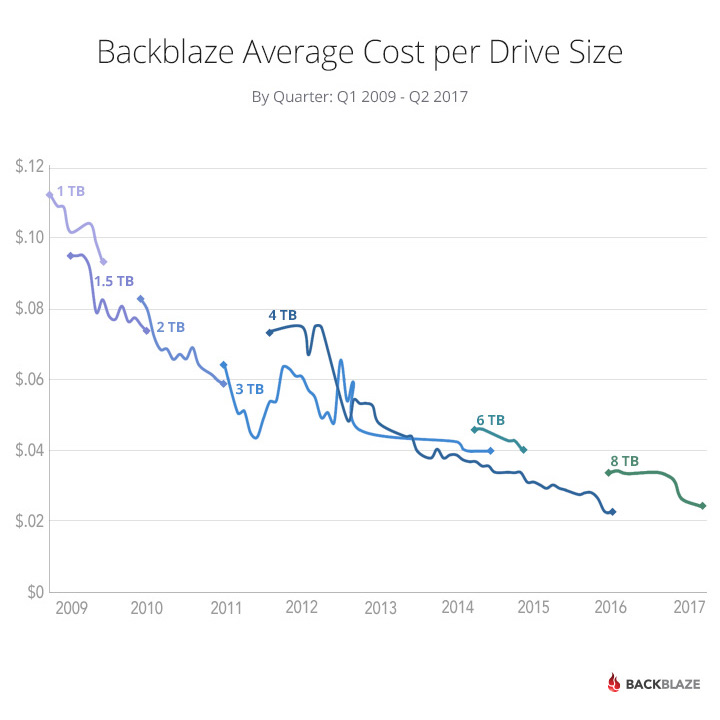
\includegraphics[height=0.6\textheight]{hdd-cost}\\
	\centering\tiny [https://www.backblaze.com/blog/hard-drive-cost-per-gigabyte/]
	\par\Large
	So, the price is low, we store everything. 
	[DRAFT]
	And i.e. if we're Facebook it's a tough question whether we should create a task for admins to create a script for housekeeping or just buy one more drive for storage.
\end{gdsw}
\begin{gdsw}
	\centering{\fontsize{30}{35pt}\selectfont\bf Information = Money}
	\par\centering\Large
	% \centering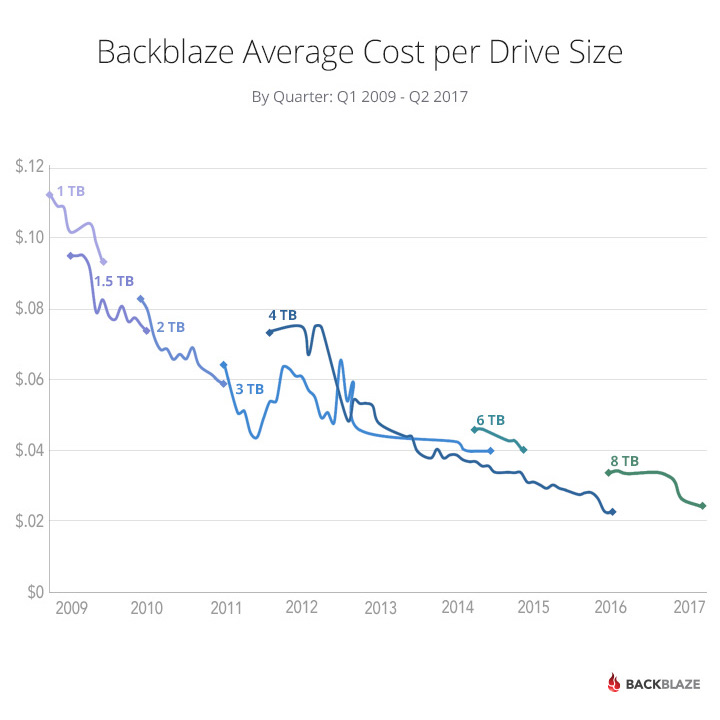
\includegraphics[width=0.7\textwidth]{hdd-cost} 
	But could we earn {\bf more} money with all of this information we collecting.\\        
\end{gdsw}
\begin{gdsw}
	\centering
\includegraphics[height=0.6\textheight]{bigdata}
	\par
	That's what basically we do in our BigData field
\end{gdsw}	
\begin{gdsw}
	\centering
\includegraphics[width=0.7\textwidth]{knight-capital}
	\par\LARGE
	Do you know this company? 
\end{gdsw}
\begin{gdsw}
	\centering
\includegraphics[width=0.7\textwidth]{knight-capital} 
	\par
	The Knight Capital Group was an American global financial services firm engaging in market making, electronic execution, and institutional sales and trading.\\
	With its high-frequency trading algorithms Knight was the largest trader in U.S.        
\end{gdsw}
\begin{gdsw}
	\centering
\includegraphics[width=0.7\textwidth]{knight-capital} 
	\par
	\begin{itemize}
		\item BigData
		\item Lot of analytics
	\end{itemize}
\end{gdsw}
\begin{gdsw}
	\centering
\includegraphics[width=0.7\textwidth]{knight-capital} 
	\par
	On August 1st, 2012, Knight Capital deployed a new software update to their production servers.
	They switched it on and immediately they started losing literally \$10 million [£6.4m] a minute.
	And this went on for 45 minutes. At the end of it all they wound up having lost \$440 million
\end{gdsw}	
\begin{gdsw}
	\centering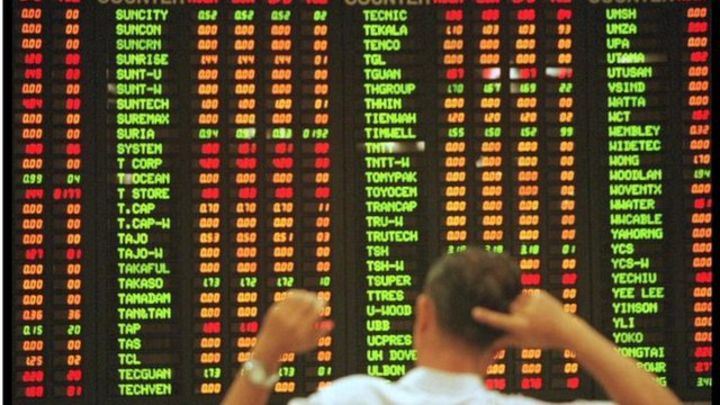
\includegraphics[width=0.7\textwidth]{trading} 
	\par
	Humans still watch the systems, but {\bf the computers move far too quickly for us to react to everything they do} - and at Knight Capital, the computer glitch meant the company was making trades it didn't intend to make. That's how to lose almost half a billion dollars in a little over half an hour.
\end{gdsw}
\begin{gdsw}
	\centering
\includegraphics[width=0.7\textwidth]{robbery2} 
	\par
	\LARGE My previous project
\end{gdsw}
\begin{gdsw}
	\centering
\includegraphics[width=0.7\textwidth]{magic} 
	\par
	\LARGE Fraud Detection System
\end{gdsw}
\begin{gdsw}
	\centering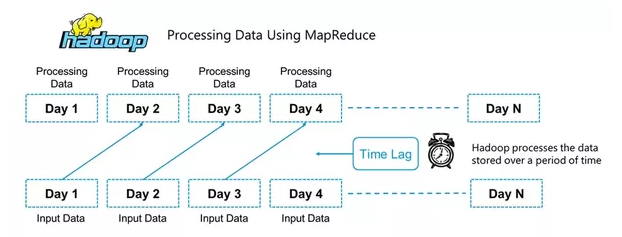
\includegraphics[height=0.6\textheight]{processing-lag} 
	\par
	\begin{center}		
		\begin{itemize}
			\item Collect - 24hrs
			\item Process - 6hrs
			\item Block Fraudsters - 10 minutes
		\end{itemize}
	\end{center}
\end{gdsw}	
\begin{gdsw}
	\centering\Large We're loosing money!\\
	
\includegraphics[height=0.7\textheight]{smart-cat} 
	\par\centering
	\pause
	30hr lag \rightarrow 70 000\$ per day
\end{gdsw}
\begin{gdsw}
	\centering{\fontsize{30}{35pt}\selectfont\bf What could be improved here?}
\end{gdsw}	
\begin{gdsw}
	\centering{\fontsize{30}{35pt}\selectfont\bf Reaction Time!}
\end{gdsw}
\begin{gdsw}
	\centering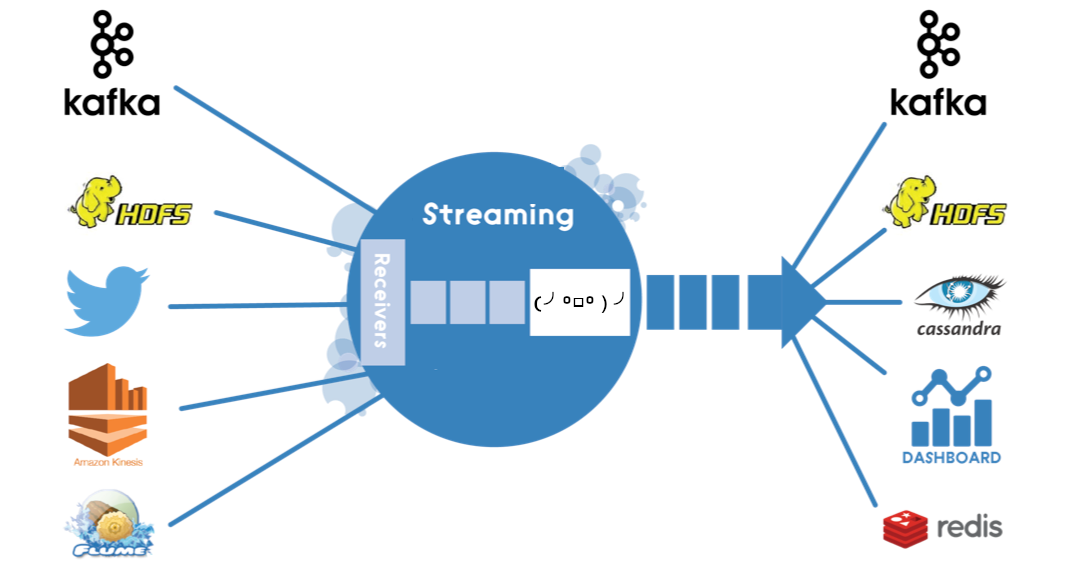
\includegraphics[height=0.7\textheight]{streaming-details} 
	\par\pause\Large
	30hr \rightarrow \Rightarrow 10mins\\
	And Fraudsters were Disappointed
\end{gdsw}
\begin{gdsw}
	\centering
\includegraphics[height=0.5\textheight]{knight-capital} 
	\par
	Was not so lucky
\end{gdsw}
\begin{gdsw}		
	\begin{columns}
		\begin{column}{0.4\textwidth}
			\centering
\includegraphics[height=0.9\textheight]{gofast} 
		\end{column}
		\begin{column}{0.6\textwidth}
			\large\centering 
			\begin{itemize}
				\item Reduce reaction time
				\item Minimize risk surface
				\item Compete for best offers in market
				\item Give out customers what they need right in time
				\item ...
			\end{itemize}	
		\end{column}
	\end{columns}
\end{gdsw}
\begin{gdsw}
	\centering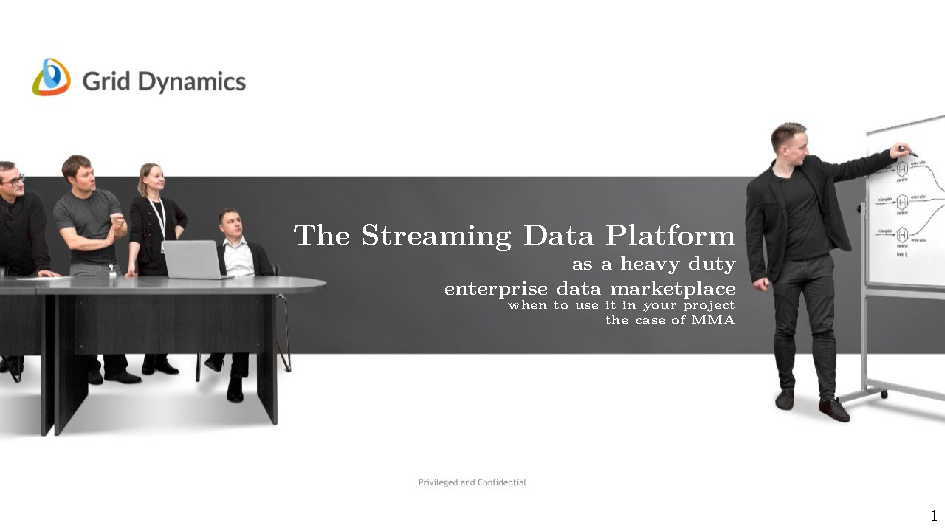
\includegraphics[height=\textheight]{sdp}         
\end{gdsw}
\begin{gdsw}
	\centering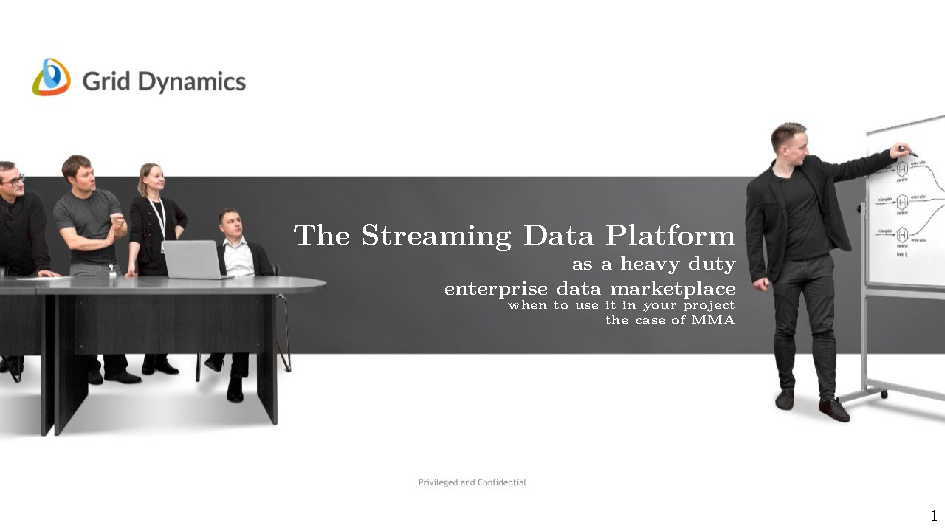
\includegraphics[height=0.5\textheight]{sdp}         
	\par
	\begin{center}
		\begin{itemize}
			\centering
			\item Improve ETL
			\item Realtime Analytics
			\item Automated Governance
			\item Superior Visualization
		\end{itemize}
	\end{center}
\end{gdsw}
\begin{gdsw}
	References:
	\begin{center}\small
		\begin{itemize}
			\item https://en.wikipedia.org/wiki/Knight\_Capital\_Group
			\item https://www.bbc.com/news/magazine-19214294
			\item https://www.backblaze.com/blog/hard-drive-cost-per-gigabyte/
		\end{itemize}
	\end{center}
\end{gdsw}
    	
\end{document}

% https://en.wikipedia.org/wiki/Knight_Capital_Group
% https://www.bbc.com/news/magazine-19214294
% For hard drive prices, the race to zero is over: nobody won. For the past 35+ years or so, hard drives prices have dropped, from around \$500,000 per gigabyte in 1981 to less than \$0.03 per gigabyte today. 


% https://www.backblaze.com/blog/hard-drive-cost-per-gigabyte/
